\documentclass{article}
\usepackage{amsmath}
\usepackage{amsthm}
\usepackage{amsfonts}
\usepackage{amssymb}
\usepackage{bbold}
\usepackage{dsfont}
\usepackage{graphicx}
\usepackage{cleveref}
\usepackage{bm}
\usepackage{booktabs}
\usepackage{siunitx}
\usepackage{xcolor}
\usepackage[utf8]{inputenc}
\usepackage[english]{babel}
\newtheorem{definition}{Definition}
\newtheorem{example}{Example}
\newcommand{\exP}[1]{\mathrm{e}^{#1}}
\newcommand{\dif}{\mathrm{d}}
\renewcommand{\vec}[1]{\mathbf{#1}}
\newcommand{\pdagger}{{\phantom{\dagger}}}
\newcommand{\state}[1]{\vert #1\rangle}
\newcommand{\cstate}[1]{\langle #1\vert}
\newcommand{\tr}[1]{\mathrm{tr}\left\{#1\right\}}
\newcommand{\trs}[2]{\, \mathrm{tr}_{#1}\{#2\}}
\newcommand{\expc}[3]{\langle #1\vert #2 \vert #3\rangle}
\usepackage[doi=false,url=false,isbn=false,backend=bibtex,style=nature,natbib=true,sorting=none]{biblatex}
\bibliography{bib.bib}
\usepackage{geometry}
\geometry{
	a4paper,
	total={170mm,257mm},
	left=20mm,
	top=20mm,
}
\begin{document}
\title{Additional results and analyses: Transport through three-site model}
\author{Rudolf Smorka}
\maketitle
%\tableofcontents
\section{Model}
\section{Parameters}
To simplify the analysis, we assume $\varepsilon_i = \varepsilon_j = \varepsilon_0$, and set the parameters to
\begin{align*}
	\varepsilon_0 &= \SI{0}{\milli\electronvolt}\\
	\omega_0 &= \SI{0.1}{\electronvolt}\\
	t_0 &= \SI{2}{\electronvolt}\\
	t_1 &= \SI{0.2}{\electronvolt}\\
	\Gamma &= \SI{10}{\milli\electronvolt}\\
	T &= \SI{5}{\milli\electronvolt}.
\end{align*} 
\section{Validity of implementation}
To check whether the implementation is valid, we consider the current dynamics through a three-site model with Peierls-terms only (no SOC, and no SOC-Phonon), and compare it to the case without spin. In the spinfull model with Peierls terms only, each eigenstate is doubly degenerate. Therefore, it is expected that the mean force exerted by the electrons on the vibrational modes is twice as large as the one in the spinless model.
\Cref{fig:Consistency_currents} shows a comparison between the symmetrized current dynamics in the spinfull model (black line) and the spinless model (red line). The current is divided by the number of levels $N$, which is $N=6$ in the spinfull case and $N=3$ in the spinless case. A comparison of the dynamics of the displacement of the bond vibration between sites 1 and 2 is shown in \cref{fig:Consistency_phonons}. Both results show an expected consistency between the spinfull and the spinless models.
\begin{figure}[!h]
	\centering
	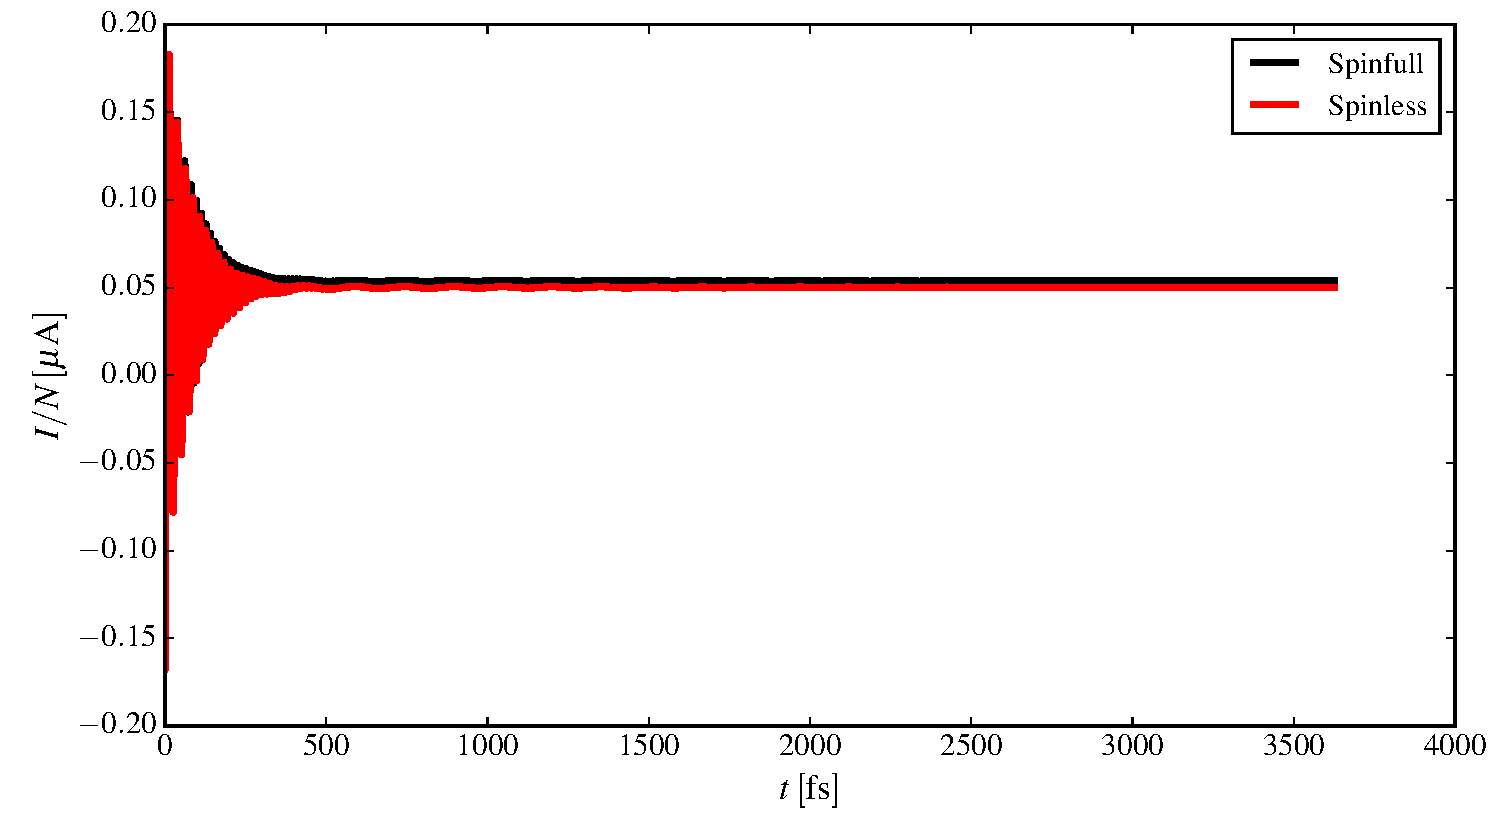
\includegraphics[width=0.8\textwidth]{figs/Peierls_L3_spin_noSpin_comparison.pdf}
	\caption{Comparison of symmetrized current divided by the number of eigenlevels: Spinfull (black line) and spinless (red line) Peierls-model with $L=3$ sites.}\label{fig:Consistency_currents}
\end{figure}
\begin{figure}[!h]
	\centering
	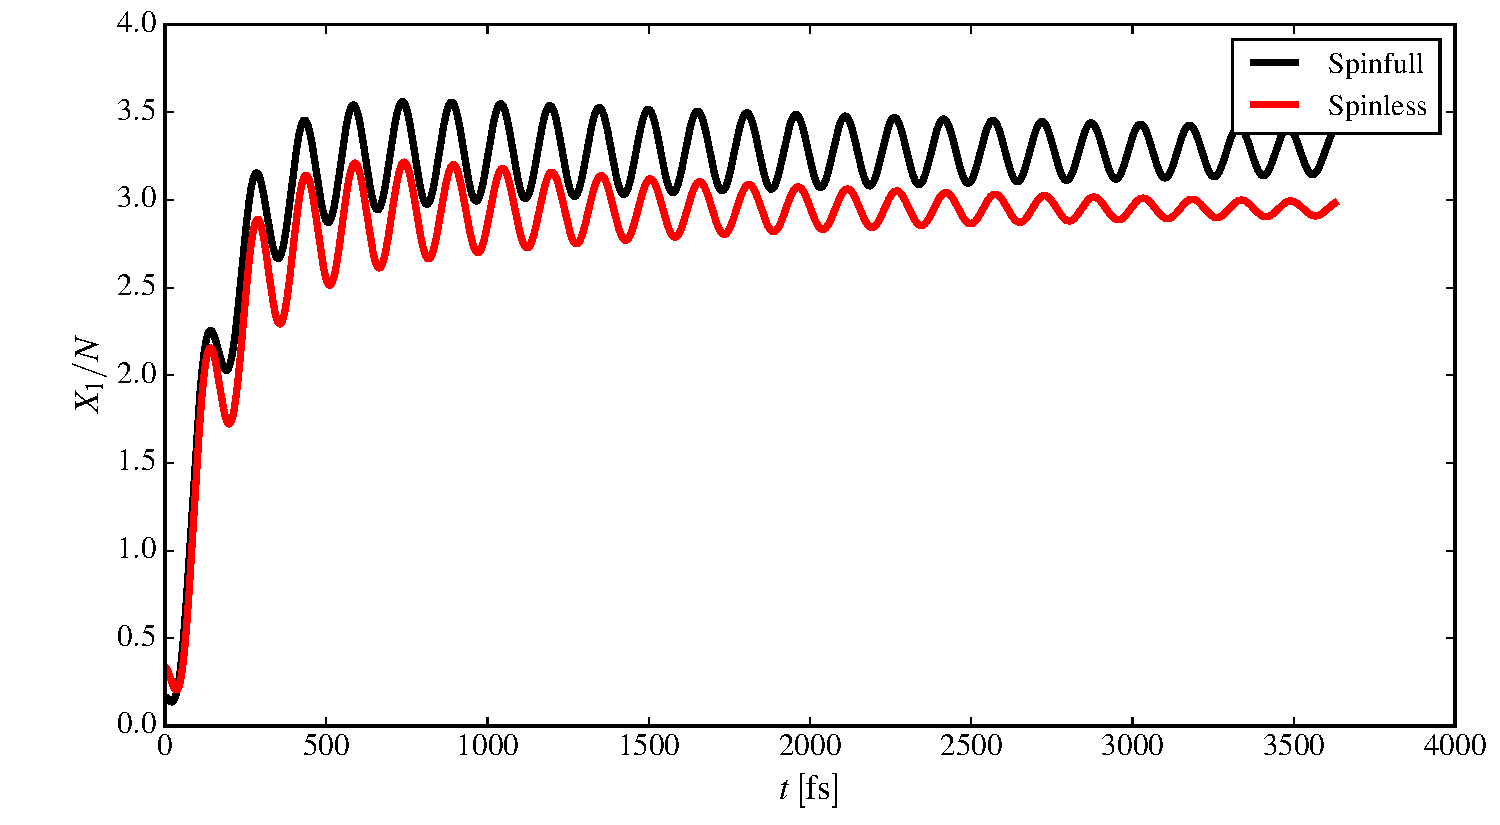
\includegraphics[width=0.8\textwidth]{figs/Peierls_L3_spin_noSpin_comparison_phonons.pdf}
	\caption{Comparison of vibrational displacement of bond mode between sites 1 and 2, divided by the number of eigenlevels: Spinfull (black line) and spinless (red line) Peierls-model with $L=3$ sites.}\label{fig:Consistency_phonons}
\end{figure}
\section{Uniqueness of the steady-state}
\subsection{Peierls model}
\begin{figure}[!h]
	\centering
	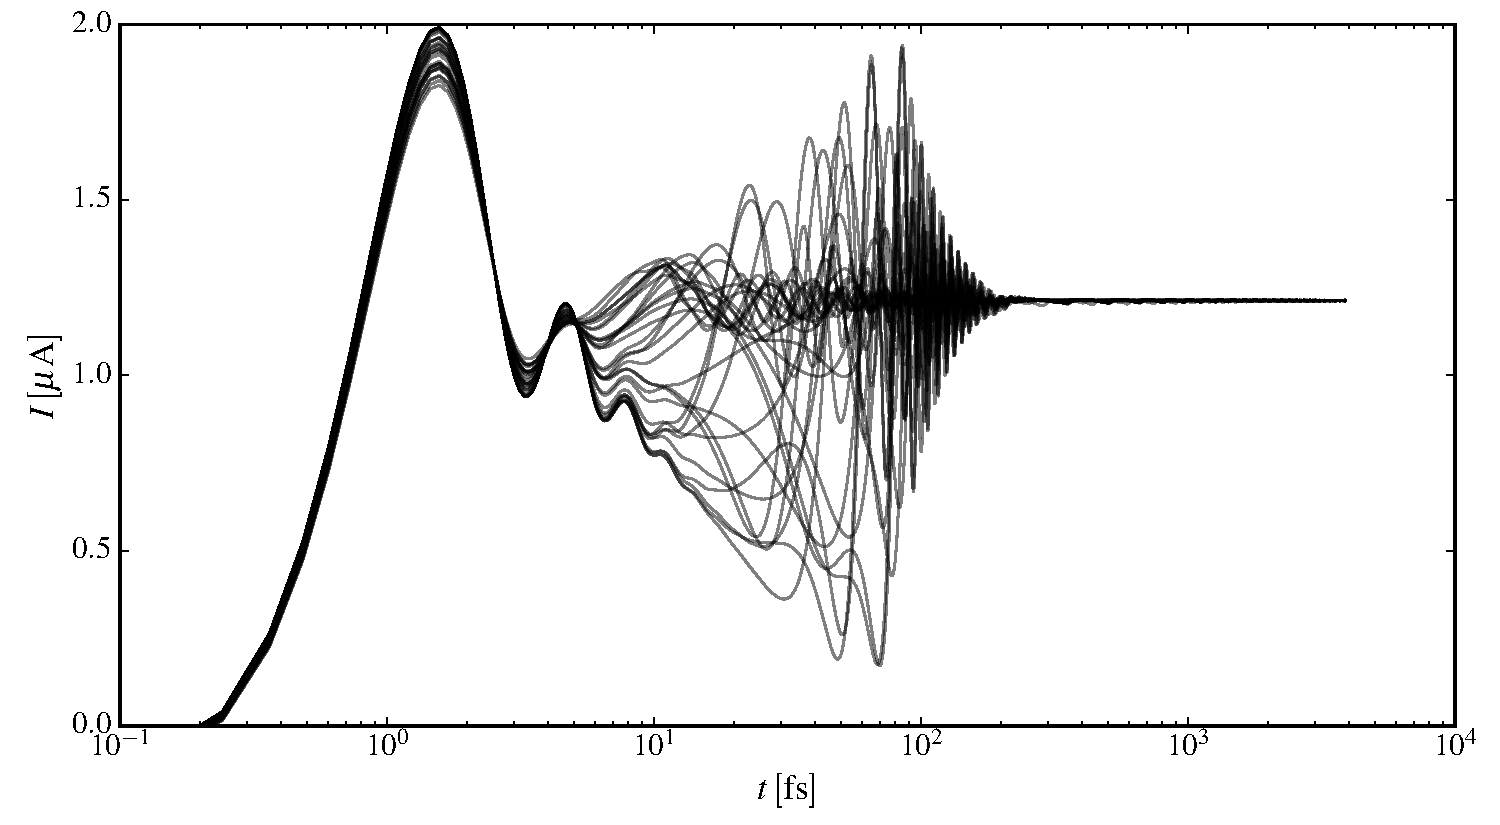
\includegraphics[width=0.9\textwidth]{figs/Fransson_L3_P0_unique_steady_state.pdf}
	\caption{Symmetrized current for $t_1 = \SI{20}{\milli\electronvolt}$, $\omega_0=\SI{10}{\milli\electronvolt}$ for different initial vibrational positions and momenta (sampled from thermal Wigner distribution).}
\end{figure}
\clearpage
\subsection{Fransson model}
\begin{figure}[!h]
	\centering
	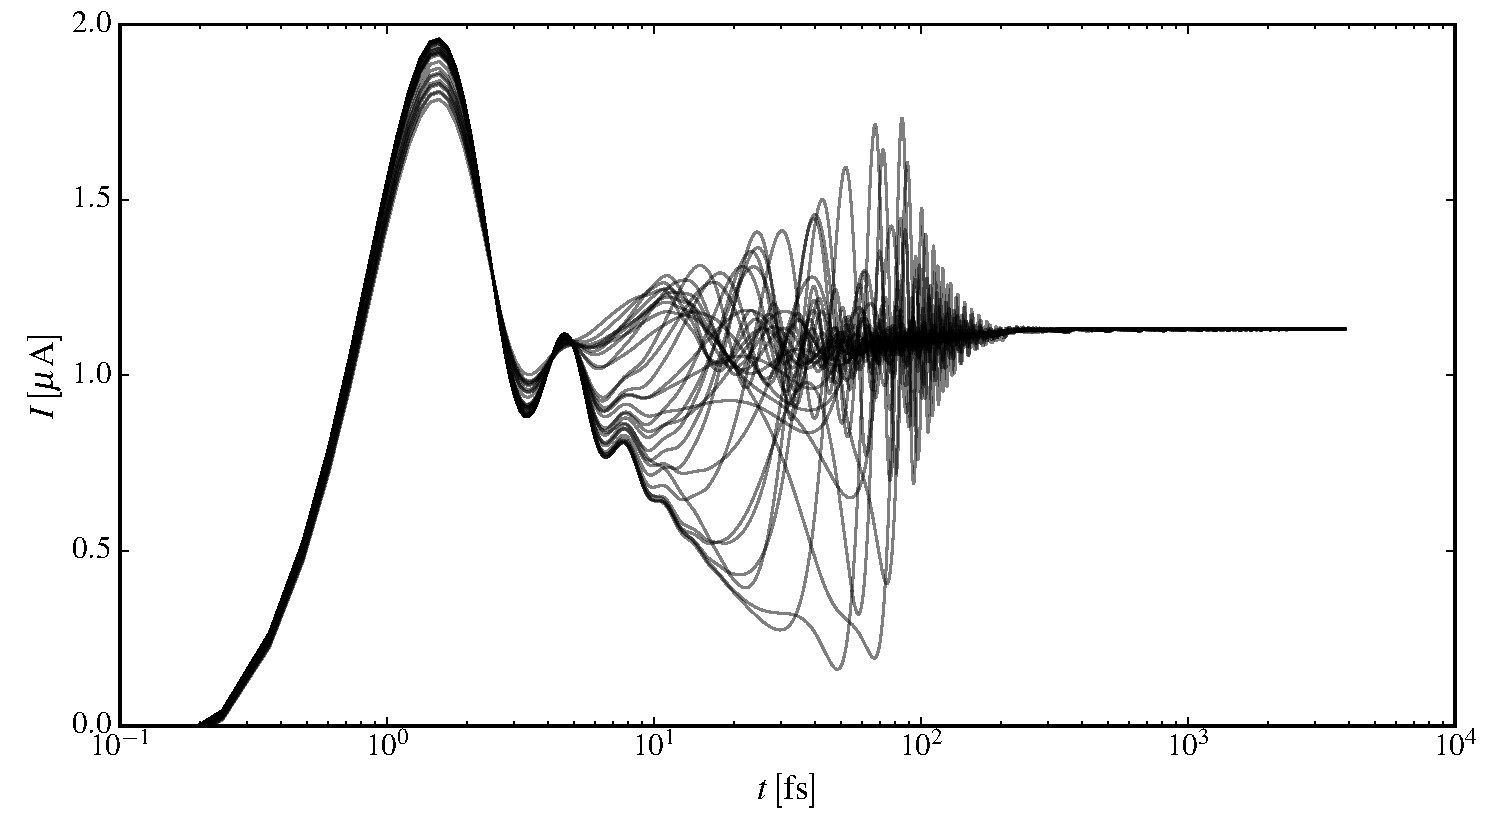
\includegraphics[width=0.9\textwidth]{figs/Fransson_L3_P0.5_unique_steady_state.pdf}
	\caption{Symmetrized current for $t_1 = \SI{20}{\milli\electronvolt}$, $\lambda_0 = \SI{1}{\milli\electronvolt}$, $\lambda_1 = \SI{1}{\milli\electronvolt}$, $\omega_0 = \SI{10}{\milli\electronvolt}$ and $P=0.5$ and different initial vibrational positions and momenta (sampled from thermal Wigner distribution).}
\end{figure}
\section{Example of non-unique steady-state}
For $L=1\times 2$ (no spin), and the following parameters
\begin{align}
	\varepsilon_0 &= \SI{-240}{\milli\electronvolt}\\
	\omega_0 &= \SI{10}{\milli\electronvolt}\\
	t_0 &= \SI{40}{\milli\electronvolt}\\
	t_1 &= \SI{40}{\milli\electronvolt}\\
	\lambda_0 &= \SI{1}{\milli\electronvolt}\\
	\lambda_1 &= \SI{0.1}{\milli\electronvolt}\\
	\Gamma &= \SI{10}{\milli\electronvolt}\\
	T &= \SI{25}{\milli\electronvolt}.
\end{align}
the system is bi-stable for some voltages. This bi-stability is also observed in larger systems with spin.

\end{document}




